\documentclass{article}
\usepackage{amsmath}
\usepackage{amssymb}
\usepackage{bm}
\usepackage{graphicx}
\usepackage{geometry}

\geometry{margin=1in}
\graphicspath{}

\title{STAT 672: Homework 3}
\author{Tom Wallace}

\begin{document}

\maketitle

\section*{SVD and Ridge Regression}

Estimated coefficients in ridge regression are given by:

$$
\hat{\bm{\beta}}_{\mathrm{ridge}} = (\mathbf{X}^T\mathbf{X} + \lambda
\mathbf{I})^{-1}\mathbf{X}^T\mathbf{y}
$$

We take the singular value decomposition of the feature matrix:

$$
= ((\mathbf{UDV}^T)^T(\mathbf{UDV}^T)+\lambda \mathbf{I})^{-1} (\mathbf{UDV}^T)^T \mathbf{y}
$$
$$
= (\mathbf{VD}^T\mathbf{U}^T\mathbf{UDV}^T + \lambda \mathbf{I})^{-1}
\mathbf{VD}^T\mathbf{U}^T \mathbf{y}
$$

We know that $\mathbf{U}^T\mathbf{U}=\mathbf{I}$ and $\mathbf{D}^T\mathbf{D}=\mathbf{D}^2$ and so can
simplify this to:
$$
= (\mathbf{VD}^2\mathbf{V}^T + \lambda \mathbf{I})^{-1} \mathbf{VDU}^T\mathbf{y}
$$

We substitute in $\mathbf{VV}^T$ for $\mathbf{I}$:

$$
= (\mathbf{VD}^2\mathbf{V}^T + \lambda \mathbf{VV}^T)^{-1} \mathbf{VDU}^T\mathbf{y}
$$

And factor out $\mathbf{VV}^T$:
$$
= \mathbf{V}(\mathbf{D}^2 + \lambda)^{-1}\mathbf{V}^T \mathbf{VDU}^T\mathbf{y}
$$

And make use of the fact that $\mathbf{V}$ is orthonormal:
$$
= \mathbf{V}(\mathbf{D}^2 + \lambda)^{-1}\mathbf{DU}^T\mathbf{y}
$$

Since $\mathbf{D}$ is diagonal, we can rewrite the expression involving it and
$\lambda$:
$$
\mathbf{D}_\lambda := (\mathbf{D}^2 + \lambda)^{-1}\mathbf{D}
$$
$$
= \mathrm{diag}\left(\frac{d_1}{d_1^2 + \lambda} \ldots \frac{d_D}{d_D^2 +
\lambda} \right)
$$

Thus, computation of estimated coefficients in ridge regression via SVD is
given by:
$$
\hat{\bm{\beta}}_{\mathrm{ridge}} = \mathbf{VD}_\lambda \mathbf{U}^T\mathbf{y}
$$
$$
\blacksquare
$$

\section*{Efficiency of Computation}

There are an inefficient method and an efficient method of re-calculating ridge
regression coefficients for a new regularization parameter $\lambda$.

In the inefficient method, we recompute the SVD every
time we update $\lambda$. SVD has complexity on the order of
$O(nd^2)$ (with $n$ corresponding to the number of rows of the feature matrix and 
$d$ corresponding to the number of columns). We then multiply $\mathbf{VD}_\lambda \mathbf{U}^T\mathbf{y}$.
A matrix-matrix product $C=AB$, where $A \in \mathbb{R}^{m \times n}$ and $B \in
\mathbb{R}^{n \times p}$, costs $2mnp$ flops. In our case, $\mathbf{U}^T \in
\mathbb{R}^{d \times n}$ and $\mathbf{Y} \in \mathbb{R}^{n \times 1}$, and so
multiplying the two costs $2 \times n \times d \times 1 = 2nd$ flops and results
in a $d \times 1$ vector. Multiplying $\mathbf{D}_\lambda \in \mathbb{R}^{d
\times d}$ and this $d \times 1$ vector costs $d$ flops (assuming we take advantage of the
diagonal structure of $\mathbf{D}_\lambda$) and results in a $d \times 1$ vector. 
Multiplying $\mathbf{V} \in \mathbb{R}^{d \times d}$ by this $d \times 1$ vector costs 
$2d^2$ flops. Adding together all these steps, we have $nd^2 + 2nd + d +
2d^2$ flops. Dropping all constant coefficients and only considering the
highest-order polynomial, we conclude that the inefficient method costs
$O(nd^2)$ flops.

A more efficient method notes that $\mathbf{D}_\lambda$ is the only part of 
$\mathbf{VD}_\lambda \mathbf{U}^T\mathbf{y}$ that depends on $\lambda$
and so we do not need to recompute the
SVD for every new value of $\lambda$. Assume that we have pre-calculated and
cached $\mathbf{U}^T\mathbf{y}$ and $\mathbf{V}$. Modifying the $d$ non-zero
values of $\mathbf{D}_\lambda$ to reflect our new value of $\lambda$ costs
$2d$ flops ($d$ flops for addition of the new $\lambda$ in the denominator, 
and $d$ flops to
divide the numerator by the new denominator). 
Computing new regression coefficients requires multiplying the new $\mathbf{D}_\lambda$ and
$\mathbf{U}^T\mathbf{y}$, which costs $2d^2$ flops, and then multiplying that
result by $\mathbf{V}$, which also costs $2d^2$ flops. Adding together these
two steps, we have $2d + 2d^2 + 2d^2$ flops. Dropping all constant coefficients and
only considering the highest-order polynomial, we conclude that the efficient method
costs $O(d^2)$ flops. 

In practical terms, since we are fitting regression coefficients on a training
dataset with $n=6000$, the efficient method is 6,000 times faster.

\section*{Results}

Below, I compare the performance of ridge and lasso regression on the homework
dataset for different values of $\lambda$. For ridge regression, a
regularization parameter value of 0.00390625 achieves the lowest test error
(2.81855); for lasso regression, a regularization parameter of $4.46e^{-0.6}$
(i.e. the tested value closest to 0) achieves the lowest test error (2.85948).
The ridge method achieves the better minimum test error. 

In the below graph, I have omitted some tested values of $\lambda$ to make
things more visually clear.

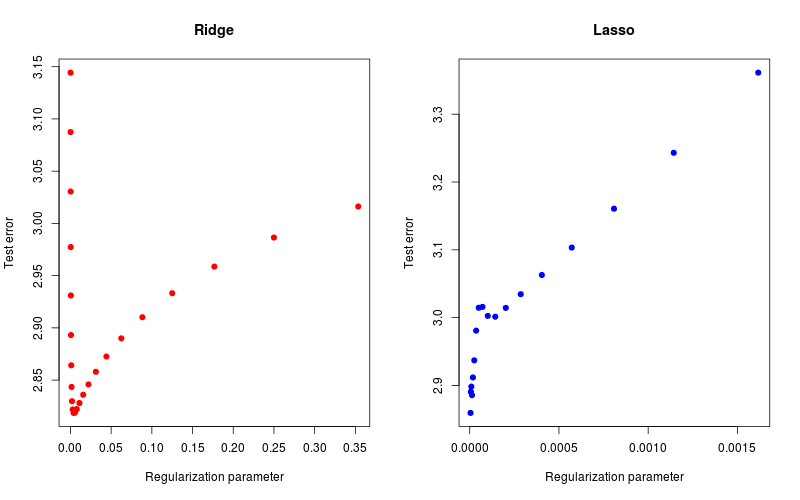
\includegraphics[scale=0.5]{foo}

\end{document}
